\section{Background and Related Work}
\label{sec:background}

We first introduce \journalv{formal} notations useful for the rest of the paper (Section~\ref{sec:notation}). Then, we review \journalv{in detail} existing time-series anomaly detection methods (Section~\ref{sec:ad_methods}), and discuss their limitations when applied to large heterogeneous sets of time series (Section~\ref{sec:limitation}). 

\subsection{Time-Series and Anomaly Score Notations}
\label{sec:notation}

\journalv{In this section, we review notations for time series and anomaly score sequences.}

\textbf{Time Series: }A time series $T \in \mathbb{R}^n $ is a sequence of real-valued numbers $T_i\in\mathbb{R}$ $[T_1,T_2,...,T_n]$, where $n=|T|$ is the length of $T$, and $T_i$ is the $i^{th}$ point of $T$. We are typically interested in local regions of the time series, known as subsequences. A subsequence $T_{i,\ell} \in \mathbb{R}^\ell$ of a time series $T$ is a continuous subset of the values of $T$ of length $\ell$ starting at position $i$. Formally, $T_{i,\ell} = [T_i, T_{i+1},...,T_{i+\ell-1}]$. \journalv{We then define a} dataset $\mathcal{D}$, which is a set of time series. Note that the time series contained in $\mathcal{D}$ can be of diverse lengths. We define the size of $\mathcal{D}$ as $|\mathcal{D}|$.

\textbf{Anomaly Score Sequence: }For a time series $T \in \mathbb{R}^n $, an anomaly detection method (or detector) $D$ returns an anomaly score sequence $S_T$. For point-based approaches (i.e., methods that return a score for each point), we have $S_T \in \mathbb{R}^n$. For subsequence-based approaches (i.e., methods that return a score for each subsequence of a given length $\ell$), we have $S_T \in \mathbb{R}^{n-\ell}$ and $S_T = [{S_T}_1,{S_T}_2,...,{S_T}_{n-\ell}]$ with ${S_T}_i \in [0,1]$. In most applications, the anomaly score has to be the same length as the time series. \journalv{Thus, for subsequence-based approaches, we define:
\begin{equation*}
    \begin{aligned}
        S_T =\, &[{S_T}_1]_{i\in[0,\ell/2]}\, + \\
                &[{S_T}_1, {S_T}_2, \ldots, {S_T}_{n-\ell}]\, + \\
                &[{S_T}_{n-\ell}]_{i\in[0,\ell/2]} \text{ with } |S_T| = |T|
    \end{aligned}
\end{equation*}
}

\textbf{Anomaly Detection Accuracy: }For a time series $T \in \mathbb{R}^n $, an anomaly detection method (or detector) $D$ that returns an anomaly score sequence $D(T) = S_T$ and labels $L \in [0,1]^n$ that indicated with 0 or 1 if the points in $T$ are normal or abnormal respectively, we define $Acc:\mathbb{R}^n,\{0,1\}^n \rightarrow [0,1]$ as an accuracy function for which $Acc(D(T),L)$ indicates how $D$ is accurate (i.e., and produce an anomaly score close to 1 when the label is equal to 1) when applied on $T$ and accordingly to $L$. The closer to one, the better.

\begin{figure}
    \centering
    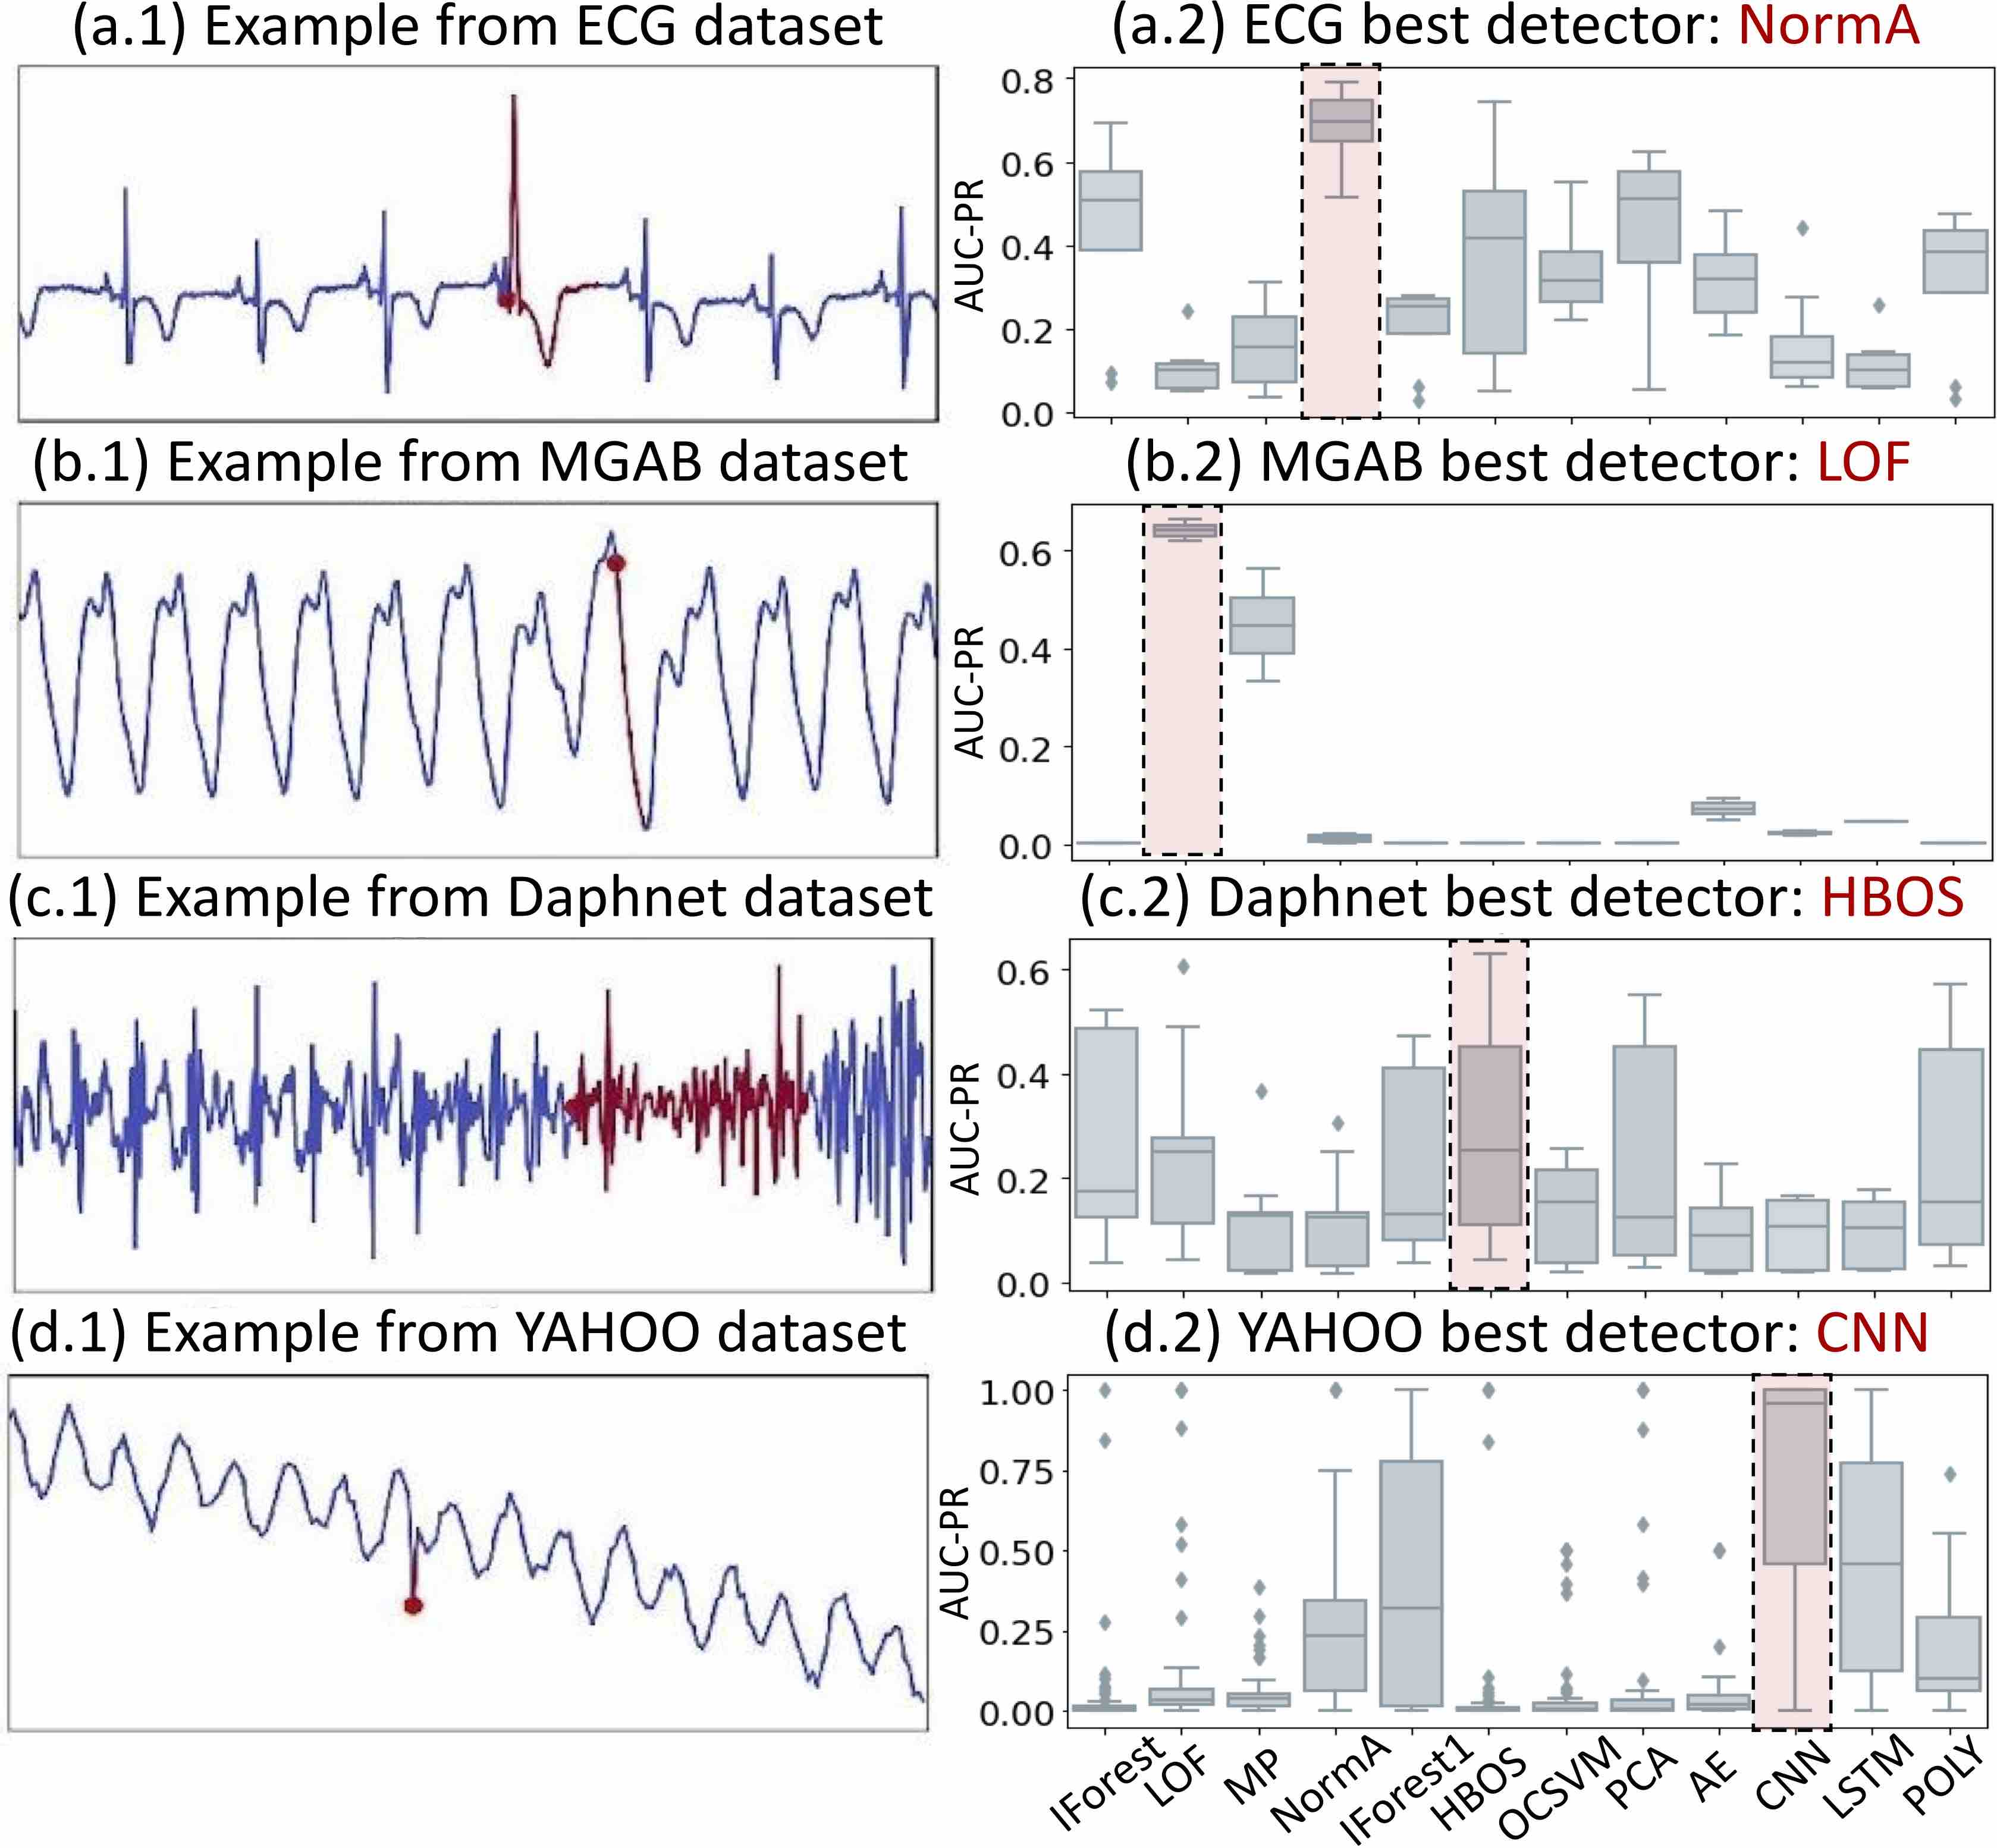
\includegraphics[width=1\linewidth]{figures/Fig2.jpg}
    \caption{Accuracy of 12 anomaly detection methods on 4 datasets.}
    \label{fig:diversity}
\end{figure}

\subsection{Anomaly Detection Methods for Time Series}
\label{sec:ad_methods}

\journalv{Anomaly detection in time series is a crucial task for many relevant applications. Therefore,} several different methods (for diverse types of time series, or applications) have been proposed in the literature. One type of anomaly detection method is \textit{discord-based methods}. These methods focus on the analysis of subsequences for the purpose of detecting anomalies in time series, mainly by utilizing nearest neighbor distances among subsequences \cite{DBLP:conf/icdm/YehZUBDDSMK16,DBLP:conf/edbt/Senin0WOGBCF15,Keogh2007,Liu2009,DBLP:conf/adma/FuLKL06,DBLP:conf/sdm/BuLFKPM07,DBLP:journals/datamine/LinardiZPK20}. 

Instead of measuring nearest neighbor distances, \textit{proximity-based methods} focus on estimating the density of particular types of subsequences in order to either extract a normal behavior or isolate anomalies. Since a subsequence can be seen as a multidimensional point (with the number of dimensions corresponding to the subsequence length), general outlier detection methods can be applied for time series anomaly detection~\cite{liu_isolation_2008,Breunig:2000:LID:342009.335388,ma2020isolation}. Among them, Isolation Forest~\cite{liu_isolation_2008} has been shown to work particularly well for time series anomaly detection task~\cite{Series2GraphPaper}. Moreover, recent proximity-based methods dedicated to identifying abnormal subsequences in time series have been proposed. For instance, NormA, a proximity-based method that first clusters data to obtain the normal behavior~\cite{norm,boniol_unsupervised_2021,DBLP:conf/icde/BoniolLRP20,boniol2021sand,boniol2021sanddemo}, \journalv{or Series2Graph that converts the time series into a graph to facilitate the detection of anomalies~\cite{Series2GraphPaper}, have both demonstrated} strong performance.

Furthermore, \textit{forecasting-based methods}, such as recurrent neural network-based ~\cite{malhotra_long_2015} or convolutional network-based ~\cite{8581424}, have been proposed for this task. Such methods use the past values as input, predict the following one, and use the forecasting error as an anomaly score. Such methods are usually trained on time series without anomalies, or make the assumption that the anomalies are significantly less frequent than the normal behaviors.

Finally, \textit{reconstruction-based methods}, such as autoencoder approaches ~\cite{10.1145/2689746.2689747}, are trained to reconstruct the time series and use the reconstruction error as an anomaly score. As both forecasting and reconstruction-based categories detect anomalies using prediction errors (either forecasting or reconstruction error), we can group them into \textit{prediction-based methods}. 

\subsection{Limitations of Anomaly Detection Methods} % on heterogeneous data}
\label{sec:limitation}

Recent benchmarks and experimental evaluations have been proposed in the literature~\cite{10.14778/3538598.3538602,10.14778/3551793.3551830,kdd21}. Such benchmarks provide a large collection of time series from various domains and evaluate multiple methods belonging to the categories mentioned above. However, these experimental evaluations led to the same conclusion: no method exists that outperforms all the others on all time series from various domains. Figure~\ref{fig:diversity}, which depicts the accuracy of 12 diverse anomaly detection methods\footnote{We use 12 methods that have been employed in previous studies ~\cite{10.14778/3529337.3529354,10.14778/3551793.3551830}. Note that other methods and variations exist that may lead to improved results.} on four time series datasets, illustrates the conclusion above. In Figure~\ref{fig:diversity} (a.2), we observe that NormA is the most accurate model on the ECG dataset~\cite{Moody} (a time series example is depicted in Figure~\ref{fig:diversity} (a.1)). However, Local Outlier Factor (LOF)~\cite{Breunig:2000:LID:342009.335388}, and Matrix profile (MP)~\cite{DBLP:conf/icdm/YehZUBDDSMK16} are significantly outperforming NormA on the MGAB dataset~\cite{markus_thill_2020_3762385} (see Figure~\ref{fig:diversity} (b.2)), whereas CNN~\cite{8581424} is outperforming NormA, LOF, and MP on the YAHOO dataset~\cite{yahoo} (see Figure~\ref{fig:diversity} (d.2)). The following two reasons explain this large difference in performance among datasets.

\subsubsection{\textbf{Heterogeneity in anomaly types}}

First, There are three types of time-series anomalies: \textit{point}, \textit{contextual}, and \textit{collective} anomalies. \textit{Point} anomalies refer to data points that deviate remarkably from the rest of the data. Similarly, \textit{Contextual} anomalies refer to data points within the expected range of the distribution (in contrast to point anomalies) but deviate from the expected data distribution, given a specific context (e.g., a window). For instance, Figure~\ref{fig:diversity} (d.1) illustrates a time series from the YAHOO dataset with a \textit{Contextual} anomaly. The value of the anomalies is inside the range of normal values, but is abnormal in the context of the distribution of values of the surrounding point. For this particular types of anomalies, \textit{reconstruction} and \textit{forcasting}-based methods are particularly accurate (as shown in Figure~\ref{fig:diversity} (d.2))

\textit{Collective} anomalies refer to sequences of points that do not repeat a typical (previously observed) pattern. The first two categories, namely, point and contextual anomalies, are referred to as \textit{point-based} anomalies, whereas \textit{collective} anomalies are referred to as \textit{subsequence} anomalies. For instance, Figure~\ref{fig:diversity} (a.1), (b.1), and (c.1) show three time series with sequence anomalies. However, even for time series belonging to the same anomaly type categories, we observe that the most accurate models are all different.  

\subsubsection{\textbf{Heterogeneity in time series structures}}

This diversity in model accuracy can be explained by other factors related to the time series structures. Indeed, on top of these categories mentioned above, the combination of them also matters. First, we need to differentiate time series containing \textit{single} anomalies from time series containing \textit{multiple} anomalies. Last, the \textit{multiple} time series category has to be divided into two subcategories, namely time series containing \textit{multiple different} and \textit{multiple similar} anomalies. For instance, methods based on neighbor distance computation such as LOF are very accurate in detecting \textit{single} or \textit{multiple different} anomalies, but less accurate for \textit{multiple similar}. To illustrate this point, Figure~\ref{fig:diversity} (a.2) depicts the results of 12 anomaly detection methods on the ECG dataset (that contains \journalv{a large number of} \textit{multiple similar} anomalies), for which LOF accuracy is low. On the contrary, Figure~\ref{fig:diversity} (b.2) depicts the results of the same 12 anomaly detection methods on the MGAB dataset (that contains \textit{multiple different} anomalies), for which LOF accuracy is high.

On top of the large variety of time series and anomaly characteristics mentioned above, time series can have distinct statistical characteristics, resulting in an even larger variability in the accuracy of anomaly detection methods. %To all these differences between time series, resulting in large variability in the accuracy of anomaly detection methods, we can add differences in the time series statistical characteristics.
The latter can be the differences between \textit{stationary} (i.e., with a constant distribution of values over time) and \textit{non-stationary} (i.e., with a changing distribution of values over time) time series, or \textit{single normality} (i.e., time series containing only one normal behavior) and \textit{multiple normalities} (i.e., time series containing multiple normal behaviors) time series. 